\documentclass[aspectratio=169,9pt]{beamer}
\mode<presentation> 
\usepackage[utf8]{inputenc}
\usepackage{sansmathaccent} %Für equations
\usepackage{amsmath}
\usepackage{tikz}
\usepackage{multicol}
\usepackage{cancel}
\usepackage{relsize}
\usepackage{graphicx}
\usepackage[table]{xcolor}
\usepackage{fontawesome5}
\usepackage[labelfont={bf},font={color=black!40,footnotesize},tablename={Tabelle},figurename={Abbildung}]{caption}
\usetikzlibrary{positioning, arrows.meta, calc}
\usefonttheme[onlymath]{serif}
%\makeatletter
%\makeatother

\rowcolors{2}{miugray!30}{miugray!10}

\usetheme{Madrid}  %% Themenwahl
\useoutertheme{split} % Alternatively: miniframes, infolines, split
%\useinnertheme{circles}


\setbeamertemplate{itemize item}{\color{miugray}$\blacksquare$}
\setbeamertemplate{itemize subitem}{\color{uniblau}$\bullet$}



\newcommand{\metermilli}{\mskip3mu \text{mm}}
\newcommand{\cm}{\mskip3mu \text{cm}}
\newcommand{\m}{ \text{m}}
\newcommand{\lite}{ \text{l}}
\newcommand{\kg}{ \text{kg}}
\newcommand{\g}{ \text{g}}
\newcommand{\km}{ \text{km}}
\newcommand{\h}{ \text{h}}
\newcommand{\s}{ \text{s}}
\newcommand{\tonne}{ \text{t}}

\newcommand{\RA}{$\rightarrow$~}
\newcommand{\pp}{\par \vspace*{2mm}}
\newcommand{\ppbig}{\par \vspace*{4mm}}

\definecolor{miudiutex}{HTML}{1d2926}
\definecolor{miugray}{HTML}{b4cccf}
\definecolor{miugray2}{HTML}{4d7365}
\definecolor{white2}{HTML}{f5f7f8}
\definecolor{red}{HTML}{cf1f5c}
\definecolor{green}{HTML}{00A36C}
\definecolor{delphinidin}{HTML}{315794}
\definecolor{uniblau}{HTML}{004e9f}
\definecolor{unigelb}{HTML}{fcba00}
\definecolor{unigrau}{HTML}{909085}
\definecolor{pelargonidin}{HTML}{b33807}
\definecolor{cyanidin}{HTML}{ba0746}
\definecolor{paeonidin}{HTML}{d15ca6}
\definecolor{petunidin}{HTML}{b56fed}
\definecolor{malvidin}{HTML}{8a2d8c}

%\setbeamercolor{palette primary}{bg=pelargonidin!35,fg=white}
%\setbeamercolor{palette secondary}{bg=delphinidin!45,fg=white}
\setbeamercolor{palette primary}{bg=uniblau!70,fg=white}
\setbeamercolor{palette secondary}{bg=uniblau!45,fg=white}
\setbeamercolor{palette tertiary}{bg=unigelb!70,fg=unigrau}
\setbeamercolor{palette quaternary}{bg=miugray,fg=white}
\setbeamercolor{structure}{fg=black} % itemize, enumerate, etc
\setbeamercolor{section in toc}{fg=red} % TOC sections

\setbeamersize{text margin left=2cm,text margin right=2cm}


\useinnertheme{tcolorbox} 
\newcommand{\goodtk}[2]{
\begin{tcolorbox}[
	enhanced,
	colframe=uniblau!75,
	sharp corners,
	boxsep=5pt,
	title=\bfseries \sffamily #1,
	colback=white,
	coltitle=black,
	attach boxed title to top text left={yshift=-\tcboxedtitleheight/2},
	boxed title style={colback=white,colframe=white}
]
	#2
	\end{tcolorbox}
}
	
\newcommand{\antwort}[1]{
\begin{tcolorbox}[
	enhanced,
	colframe=unigrau!65,
	sharp corners,
	boxsep=1pt,
	colback=white,
	coltitle=black,
]
	#1
	\end{tcolorbox}
}


\title{3. Übung}
\author{PD Dr. Helene Loos}
\date{\today}

\begin{document}
%\maketitle
\small



\begin{frame}
\begin{center}

\LARGE Übung 3  \par \normalsize
Prozessbezogene Lebensmitteltechnologie
\end{center}
\small
\end{frame}

\begin{frame}
Nachtrag letzte Stunde:
\begin{itemize}
\item In der Klausur: Erdanziehung 9,81 m/s$^2$
\end{itemize}
\end{frame}

\begin{frame}
\begin{minipage}{.4\textwidth}
{\color{miugray}$\blacksquare ~$} \textbf{Aufgabe 1} \par \vspace*{2mm}
Öl mit einer Viskosität von 0,031 kg/m$\cdot$s und einer Dichte von 850 kg/m$^3$ soll mit 13 m$^3$/h bei einem zulässigen Druckabfall von 0,1 bar laminar durch ein kreisrundes Rohr der Länge $l$ = 100 m geleitet werden. \par 
\begin{itemize}
\item Wie groß ist die Nennweite?
\item Ist die Annahme einer laminaren Strömungsform berechtigt?
\end{itemize}
 
\end{minipage}%
\hspace*{4mm}
\begin{minipage}{.6\textwidth}
\antwort{
\uncover<2->{Druckverlust durch Reibung:}
\uncover<3->{
\begin{align*}
 \Delta p &=  \frac{8 \eta \cdot \Delta l}{\pi \cdot r^4} \cdot \dot{V} \\
\end{align*}}
\uncover<4->{
Umformen:
\begin{align*}
r^4 &=  \frac{8 \eta \cdot \Delta l}{\pi \cdot  \Delta p} \cdot \dot{V} \\
r &= \sqrt[4]{\frac{8 \eta \cdot \Delta l}{\pi \cdot  \Delta p} \cdot \dot{V}}
\end{align*}
}
}
\end{minipage}%
\end{frame}

\begin{frame}
\begin{minipage}{.4\textwidth}
{\color{miugray}$\blacksquare ~$} \textbf{Aufgabe 1} \par \vspace*{2mm}
Öl mit einer Viskosität von 0,031 kg/m$\cdot$s und einer Dichte von 850 kg/m$^3$ soll mit 13 m$^3$/h bei einem zulässigen Druckabfall von 0,1 bar laminar durch ein kreisrundes Rohr der Länge $l$ = 100 m geleitet werden. \par 
\begin{itemize}
\item Wie groß ist die Nennweite?
%\item Ist die Annahme einer laminaren Strömungsform berechtigt?
\end{itemize}
 
\end{minipage}%
\hspace*{4mm}
\begin{minipage}{.6\textwidth}
\antwort{
\uncover<2->{
Werte einsetzen:}
\begin{align*}
\uncover<3->{r &= \sqrt[4]{\frac{8 \cdot 0,031 ~\text{kg/ms} \cdot 100~\text{m}}{\pi \cdot  0,1 \text{bar}} \cdot 13~\text{m}^3/\text{h}} \\}
\uncover<4->{r &= \sqrt[4]{\frac{8 \cdot 0,031 ~\text{kg/ms} \cdot 100~\text{m}}{\pi \cdot  10.000 ~\text{kg/ms}^2} \cdot 0,00361~\text{m}^3/\text{s}}\\}
\uncover<5->{r &\approx 0,041~\text{m} \\
d &\approx 0,082~\text{m} \\
d &\approx 8,2~\text{cm}}
\end{align*}
}
\end{minipage}%
\end{frame}
\begin{frame}
\begin{minipage}{.4\textwidth}
{\color{miugray}$\blacksquare ~$} \textbf{Aufgabe 1} \par \vspace*{2mm}
Öl mit einer Viskosität von 0,031 kg/m$\cdot$s und einer Dichte von 850 kg/m$^3$ soll mit 13 m$^3$/h bei einem zulässigen Druckabfall von 0,1 bar laminar durch ein kreisrundes Rohr der Länge $l$ = 100 m geleitet werden. \par 
\begin{itemize}
%\item Wie groß ist die Nennweite?
\item Ist die Annahme einer laminaren Strömungsform berechtigt?
\end{itemize}
 
\end{minipage}%
\hspace*{4mm}
\begin{minipage}{.6\textwidth}
\antwort{
Strömung auf Turbulenz prüfen:
\uncover<2->{\begin{align*}
\text{Re}_{\text{krit}} = \frac{\rho d v}{\eta} = 2.300
\end{align*}}
\uncover<3->{$v$ ausrechnen:
\begin{align*}
v = \frac{\dot{V}}{A} \rightarrow \qquad }v &= \uncover<4->{\frac{13~\text{m}^3/\text{h}}{\pi \cdot (0,041~\text{m})^2} \\
&= 2461,65~\text{m/h} \\
&= 0,684~\text{m/s} }
\end{align*}
\uncover<5->{
Werte einsetzen:}
\uncover<6->{
\begin{align*}
Re &= \frac{850~\text{kg/m}^3 \cdot 0,082~\text{m} \cdot 0,684~\text{m/s}}{0,031~\text{kg/ms}}\\
&\approx 1537,9}\uncover<7->{ \rightarrow {laminar}}
\end{align*}


}
\end{minipage}%

\end{frame}


\begin{frame}
\begin{minipage}{.4\textwidth}
{\color{miugray}$\blacksquare ~$} \textbf{Aufgabe 2} \par \vspace*{2mm}
\small
Wasser von 20 °C ($\eta$ = 10$^{-3}$ Pa s ; $\rho$ = 1.000 kg/m$^3$) fließt mit einem Volumenstrom von 600 m$^3$/h durch ein Stahlrohr ($\xi$ = 0,0113) mit der Nennweite 200 mm. \par 
\begin{itemize}
\item Wie groß ist der Druckverlust bei einer Leitungslänge von 1.000 m?
%\item Wenn die Rohrreibungszahl nicht angegeben wäre, wie könnten Sie diese herausfinden?
%\item Welche Faktoren fließen in die Rohrreibungszahl ein?
\end{itemize}

\end{minipage}%
\hspace*{4mm}
\begin{minipage}{.6\textwidth}
\antwort{
\footnotesize
\uncover<2->{
$\overline{v}$ ausrechnen:}
\uncover<3->{
\begin{align*}
\overline{v} = \frac{\dot{V}}{A} \rightarrow \overline{v} &= \frac{600~ \m^3/\text{h}}{\pi \cdot (0,1 \mskip3mu \text{m})^2} \\
 &\approx 19.098,6~\text{m/h} \\
 &\approx 5,3~\text{m/s}  \\ \\
\end{align*}
}
\uncover<4->{
Wir nutzen die Formel für Druckabfall im Rohr:}
\uncover<5->{
\begin{align*}
\Delta p &= \xi \cdot \frac{l}{d} \cdot \frac{1}{2} \rho \cdot \overline{v}^2\\
\end{align*}
}
\uncover<6->{
Werte einsetzen:}
\uncover<7->{
\begin{align*}
\Delta p &= 0,0113 \cdot \frac{1.000~\text{m}}{0,2~\text{m}} \cdot \frac{1}{2} \cdot 1.000 ~\text{kg/m}^3 \cdot (5,3~\text{m/s})^2 \\ &\approx 793.542~\text{Pa}\\
&\approx 7,94 \text{bar}
\end{align*}
}
}
\end{minipage}%
\end{frame}



\begin{frame}
\begin{minipage}{.35\textwidth}
{\color{miugray}$\blacksquare ~$} \textbf{Aufgabe 2} \par \vspace*{2mm}
Wasser von 20 °C ($\eta$ = 10$^{-3}$ Pa s ; $\rho$ = 1.000 kg/m$^3$) fließt mit einem Volumenstrom von 600 m$^3$/h durch ein Stahlrohr ($\xi$ = 0,0113) mit der Nennweite 200 mm. \par 
\begin{itemize}
%\item Wie groß ist der Druckverlust bei einer Leitungslänge von 1.000 m?
\item Wenn die Rohrreibungszahl nicht angegeben wäre, wie könnten Sie diese herausfinden?
\item Welche Faktoren fließen in die Rohrreibungszahl ein?
\end{itemize}

\end{minipage}%
\hspace*{4mm}
\begin{minipage}{.65\textwidth}
\antwort{
\uncover<2->{
Über zum Teil aufwendige Gleichungen (Colebrook,
Nikuradse, etc.) oder aber über das Auslesen eines
Moody-Diagramms.
\pp}
\uncover<3->{
Die Rohrreibungszahl ist Abhängig von:
\begin{itemize}
\item relativer Rauhigkeit $e$ (Quotient aus Wandrauhigkeit
und Rohrinnendurchmesser k/d)
\item Reynoldszahl

\end{itemize}
}
}
\end{minipage}%
\end{frame}


\begin{frame}
\begin{minipage}{.5\textwidth}
{\color{miugray}$\blacksquare ~$} \textbf{Aufgabe 3} \par \vspace*{2mm}
Der Volumenstrom von Bier, das durch ein Rohr fließt, beträgt 1,8 L/s. Der
Innendurchmesser des Rohres beträgt 3 cm. Das Bier hat eine Dichte von 1.100 kg/m$^3$.

\begin{itemize}
\item Berechnen Sie die durchschnittliche Geschwindigkeit von Bier in m/s und seinen Massendurchfluss in kg/s.
\item Wie hoch ist die Geschwindigkeit bei gleichem Volumenstrom, wenn ein anderes Rohr mit einem Durchmesser von 1,5 cm verwendet wird?
\end{itemize}

\end{minipage}%
\hspace*{4mm}
\begin{minipage}{.5\textwidth}
\antwort{
$\dot{V} = 1,8 ~$L$/$s $ = 0,0018~$m$^3/$s \par 
$r=0,015~$m \pp
Massendurchfluss:
\begin{align*}
0,0018~\m^3/\s \cdot 1100~\kg/\m^3 = 1,98~\kg/\s
\end{align*}
Mittlere Geschwindigkeiten für versch. Durchmesser:
\begin{align*}
\overline{v} &= \frac{\dot{V}}{A} \\ 
\overline{v} &= \frac{0,0018~\m^3/s}{\pi \cdot (0,015~\text{m})^2} \qquad = 2,546~\m/\s \\
\overline{v} &= \frac{0,0018~\m^3/\s}{\pi \cdot (0,0075~\text{m})^2} \qquad = 10,19~\m/\s \\
\end{align*}
}
\end{minipage}%
\end{frame}

\begin{frame}

\begin{center}
\href{https://www.youtube.com/watch?v=B6h5pVETbd8}{{\color{red}\faYoutube} Youtube-Video}
\end{center}
\end{frame}


\begin{frame}

{\color{miugray}$\blacksquare ~$} \textbf{Aufgabe 4} \par \vspace*{2mm}

\begin{tikzpicture}[scale=3]


\node(a)at(0,0){
\begin{tikzpicture}[scale=2]
\node[align=center,scale=1](1)at(0.5,1.5){Newtonsch};
\draw (0,1)node[right]{$\tau$} -- (0,0) -- (1,0)node[right,scale=0.8]{$\dot{\gamma}$};
\draw[yshift=-1.5cm] (0,1)node[right]{$\eta$} -- (0,0) -- (1,0)node[right,scale=0.8]{$\dot{\gamma}$};

\uncover<2->{\draw[black!80] (0,0) -- (0.9,0.9);}
\uncover<3->{\draw[black!80,yshift=-1.5cm] (0,0.5) -- (0.9,0.5);}

\end{tikzpicture}
};
\node(b)at(1,0){
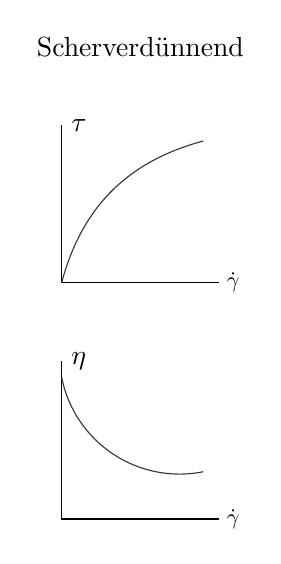
\begin{tikzpicture}[scale=2]
\node[align=center,scale=1](1)at(0.5,1.5){Scherverdünnend};
\draw (0,1)node[right]{$\tau$} -- (0,0) -- (1,0)node[right,scale=0.8]{$\dot{\gamma}$};
\draw[yshift=-1.5cm] (0,1)node[right]{$\eta$} -- (0,0) -- (1,0)node[right,scale=0.8]{$\dot{\gamma}$};


\uncover<4->{\draw[black!80] (0,0) to [bend left=30] (0.9,0.9);}
\uncover<5->{\draw[black!80,yshift=-1.5cm] (0,0.9) to [bend right=45] (0.9,0.3);}


\end{tikzpicture}
};
\node(c)at(2.1,0){
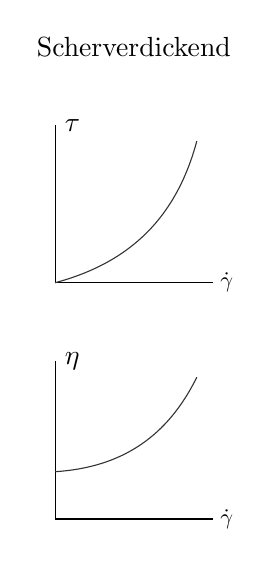
\begin{tikzpicture}[scale=2]
\node[align=center,scale=1](1)at(0.5,1.5){Scherverdickend};
\draw (0,1)node[right]{$\tau$} -- (0,0) -- (1,0)node[right,scale=0.8]{$\dot{\gamma}$};
\draw[yshift=-1.5cm] (0,1)node[right]{$\eta$} -- (0,0) -- (1,0)node[right,scale=0.8]{$\dot{\gamma}$};

\uncover<6->{\draw[black!80] (0,0) to [bend right=30] (0.9,0.9);}
\uncover<7->{\draw[black!80,yshift=-1.5cm] (0,0.3) to [bend right=30] (0.9,0.9);}

\end{tikzpicture}
};
\node[scale=0.9,rotate=90](fl)at(-0.75,0.45){Fließkurve};
\node[scale=0.9,rotate=90,align=left](vi)at(-0.75,-0.65){Viskositäts-\\kurve};
\end{tikzpicture}



\end{frame}



\begin{frame}

\begin{minipage}{.5\textwidth}
{\color{miugray}$\blacksquare ~$} \textbf{Aufgabe 5} \par \vspace*{2mm}
In der Abbildung rechts können Sie den Aufbau eines Pumpensystems mit Rohrleitungen und diversen Bauteilen sehen.
 
\begin{itemize}
\item Ermitteln Sie die mittlere Strömungsgeschwindigkeit in der Rohrleitung.
\item Bestimmen Sie die Reynoldszahl der Rohrströmung und aus dem Moody Diagramm die Rohrreibungszahl $\xi$.
\item Wie groß ist der Gesamtdruckverlust der Rohrleitung? (Beschleunigungsdruckverlust kann hier vernachlässigt werden)
\item Welchen Druck muss die Pumpe aufbauen? 
\item Wie groß ist die mechanische Antriebsleistung der Pumpe? 
\end{itemize}





\end{minipage}%
\hspace*{4mm}
\begin{minipage}{.5\textwidth}


\begin{figure}[h]
\resizebox{.7\textwidth}{!}{

\begin{tikzpicture}[>=Stealth, font=\sffamily, line width=1pt]

% --- Colors for handwritten notes ---
\colorlet{pencolor}{black!50}

% --- Macros ---
% Macro for the water level symbol
\newcommand{\waterlevel}[2]{
    \begin{scope}[shift={(####1,####2)}]
        \draw[line width=1pt] (-0.3, 0) -- (0.3, 0);
        \draw[line width=1pt] (0, 0) -- (-0.15, 0.25) -- (0.15, 0.25) -- cycle;
        \draw[line width=1pt] (-0.2, 0.25) -- (0.2, 0.25);
        \draw[line width=1pt,rotate=90,xshift=-4pt,yshift=-10.2pt] (-0.15, 0.4) .. controls (-0.05, 0.4) and (0.05, 0.3) .. (0.15, 0.4);
    \end{scope}
}

% Macro for a vertical valve (Bow-tie with T-handle)
\newcommand{\valveV}[2]{
    \begin{scope}[shift={(####1,####2)}]
        \draw[line width=1pt, fill=white] (-0.2, -0.3) -- (0.2, 0.3) -- (-0.2, 0.3) -- (0.2, -0.3) -- cycle;
        \draw[line width=1pt] (0, 0) -- (0.4, 0);
        \draw[line width=1pt] (0.4, -0.15) -- (0.4, 0.15);
    \end{scope}
}

% --- Tanks ---
% Tank 1 (Left, open)
\draw (0, 3) -- (0, 0) -- (3, 0) -- (3, 3);
\draw (0, 1.5) -- (3, 1.5); % Water surface
\waterlevel{1.5}{1.5}


% Tank 2 (Right Top, closed cylinder)
\begin{scope}[shift={(7, 8)}]
    \draw (-2.5, -1) -- (1.25, -1);
    \draw (-2.5, 1) -- (1.25, 1);
    \draw (-2.5, -1) arc (270:90:0.5 and 1);
    \draw (1.25, -1) arc (-90:90:0.5 and 1);
    
    \draw (-2.9, 0.5) -- (1.65, 0.5); % Water surface inside
    \waterlevel{1}{0.5}
    \node[align=left] at (0, -0.2) {$p_B = 2 \text{ bar}$\\ Überdruck};
\end{scope}

% --- Pipes ---
\draw (1.5, 0) -- (1.5, -1.7) -- (1.5, -1.7) to[bend right=45] (1.8, -2)--(3.7,-2) to[bend left=45] (4,-2.3) -- (4, -2.3)  -- (4, -3.7) to[bend right=45]  (4.3, -4);
% Path from Pump to Tank 2
\draw (4, -4) -- (6.7, -4) to[bend right=45] (7, -3.7)-- (7, 7);

% --- Pump ---
\draw[fill=white,xshift=-1.4cm] (5.5, -4) circle (0.5);
% Pump inner triangle symbol (flow direction)
%\draw (5.2, -4.2) -- (5.8, -4.2) -- (5.5, -3.6) -- cycle;
\draw[xshift=-1.4cm] (5.5,-3.5) -- (6,-4);
\draw[xshift=-1.4cm] (5.5,-4.5) -- (6,-4);

% --- Break in vertical pipe ---
\fill[white] (6.5, 2.3) rectangle (7.5, 2.7);
\draw (6.8, 2.2) -- (7.2, 2.4);
\draw (6.8, 2.6) -- (7.2, 2.8);

% --- Valves ---
\valveV{1.5}{-1}     % Under Tank 1
\valveV{4}{-3}       % Before Pump
\valveV{7}{-2.5}     % After Pump
\valveV{7}{6}        % Before Tank 2

% --- Dimensions and Labels ---
% 5m height dimension
\draw[thin] (3, 1.5) -- (5.5, 1.5);
\draw[<->] (5, 1.5) -- (5, 8.5) node[midway, fill=white] {5 m};


% "90° Krümmer" and circle
\node[pencolor, right] at (5.5, -4.8) {90$^\circ$ Rohrbogen};
\draw[pencolor, thin, dashed] (6.9, -3.9) circle (0.4); 



\end{tikzpicture}
} 
\caption{Modell des Rohrleitungssystems}
%\caption{Modell des Rohrleitungssystems.\\
% \symPumpe~Pumpe, 
% \\
% \symVentil~Absperrventil, \\ \symBogen~$90^\circ$-Rohrbogen.}
%\label{rohr}
\end{figure}

\end{minipage}%

\end{frame}




\begin{frame}





\begin{minipage}{.5\textwidth}
\begin{table}[h]
%\caption{Werte für Aufgabe 5}
\resizebox{\textwidth}{!}{
\begin{tabular}{ll}
    $\dot{V}$&$= 18 \text{ m}^3\text{/h}$ \\ \hline
     Rohrbögen 90$^\circ$ $\zeta $&$= 0,2$ \\ \hline
    Gesamtrohrlänge $l $&$= 8 \text{ m}$ \\ \hline
    Einlauf scharfkantig $\zeta$&$ = 0,5$ \\ \hline
    Rohrrauheit $k/d$ &$=1/2.000$ \\ \hline
    Ventil $\zeta $&$= 0,8$ \\ \hline
    Viskosität von Wasser $\nu $&$= 1 \cdot 10^{-6} \text{ m}^2\text{/s}$ \\ \hline Rohrdurchmesser&$=60.3 \text{ mm}$ \\ \hline
$\rho $&$= 1.000 \text{ kg/m}^3$    \\ \hline
 Wandstärke $s $&$=2.9 \text{ mm}$ 
\end{tabular}
}
\end{table}

\end{minipage}%
\hspace*{4mm}
\begin{minipage}{.5\textwidth}
\antwort{
\textbf{Mittlere Strömungsgeschwindigkeit:}

\uncover<2->{
\begin{align*}
\dot{V} &= \overline{v} \cdot A \\
\overline{v} &= \frac{\dot{V}}{A} \\
\overline{v} &= \frac{\dot{V}}{\pi \cdot \left(\frac{d_i}{2}\right)^2 }
\end{align*}}
\uncover<3->{
Innendurchmesser berechnen:
\begin{align*}
d_i &= d_a - 2 \cdot s \\
	&= 60,3~\text{mm} - 2 \cdot 2,4~\text{mm} = 54,5 ~\text{mm}
\end{align*}
}
\uncover<4->{
Einsetzen:
\begin{align*}
\overline{v} &= \frac{18~\text{m}^3}{3.600~\text{s} \cdot \pi \cdot \left(\frac{54,5\cdot 10^{-3}~\text{m}}{2}\right)^2}\\
&=2,143~\text{m/s}
\end{align*}
}}
\end{minipage}%

\end{frame}


\begin{frame}





\begin{minipage}{.4\textwidth}
\begin{figure}[h]
\resizebox{.9\textwidth}{!}{

\begin{tikzpicture}[>=Stealth, font=\sffamily, line width=1pt]

% --- Colors for handwritten notes ---
\colorlet{pencolor}{black!50}

% --- Macros ---
% Macro for the water level symbol
\newcommand{\waterlevel}[2]{
    \begin{scope}[shift={(####1,####2)}]
        \draw[line width=1pt] (-0.3, 0) -- (0.3, 0);
        \draw[line width=1pt] (0, 0) -- (-0.15, 0.25) -- (0.15, 0.25) -- cycle;
        \draw[line width=1pt] (-0.2, 0.25) -- (0.2, 0.25);
        \draw[line width=1pt,rotate=90,xshift=-4pt,yshift=-10.2pt] (-0.15, 0.4) .. controls (-0.05, 0.4) and (0.05, 0.3) .. (0.15, 0.4);
    \end{scope}
}

% Macro for a vertical valve (Bow-tie with T-handle)
\newcommand{\valveV}[2]{
    \begin{scope}[shift={(####1,####2)}]
        \draw[line width=1pt, fill=white] (-0.2, -0.3) -- (0.2, 0.3) -- (-0.2, 0.3) -- (0.2, -0.3) -- cycle;
        \draw[line width=1pt] (0, 0) -- (0.4, 0);
        \draw[line width=1pt] (0.4, -0.15) -- (0.4, 0.15);
    \end{scope}
}

% --- Tanks ---
% Tank 1 (Left, open)
\draw (0, 3) -- (0, 0) -- (3, 0) -- (3, 3);
\draw (0, 1.5) -- (3, 1.5); % Water surface
\waterlevel{1.5}{1.5}


% Tank 2 (Right Top, closed cylinder)
\begin{scope}[shift={(7, 8)}]
    \draw (-2.5, -1) -- (1.25, -1);
    \draw (-2.5, 1) -- (1.25, 1);
    \draw (-2.5, -1) arc (270:90:0.5 and 1);
    \draw (1.25, -1) arc (-90:90:0.5 and 1);
    
    \draw (-2.9, 0.5) -- (1.65, 0.5); % Water surface inside
    \waterlevel{1}{0.5}
    \node[align=left] at (0, -0.2) {$p_B = 2 \text{ bar}$\\ Überdruck};
\end{scope}

% --- Pipes ---
\draw (1.5, 0) -- (1.5, -1.7) -- (1.5, -1.7) to[bend right=45] (1.8, -2)--(3.7,-2) to[bend left=45] (4,-2.3) -- (4, -2.3)  -- (4, -3.7) to[bend right=45]  (4.3, -4);
% Path from Pump to Tank 2
\draw (4, -4) -- (6.7, -4) to[bend right=45] (7, -3.7)-- (7, 7);

% --- Pump ---
\draw[fill=white,xshift=-1.4cm] (5.5, -4) circle (0.5);
% Pump inner triangle symbol (flow direction)
%\draw (5.2, -4.2) -- (5.8, -4.2) -- (5.5, -3.6) -- cycle;
\draw[xshift=-1.4cm] (5.5,-3.5) -- (6,-4);
\draw[xshift=-1.4cm] (5.5,-4.5) -- (6,-4);

% --- Break in vertical pipe ---
\fill[white] (6.5, 2.3) rectangle (7.5, 2.7);
\draw (6.8, 2.2) -- (7.2, 2.4);
\draw (6.8, 2.6) -- (7.2, 2.8);

% --- Valves ---
\valveV{1.5}{-1}     % Under Tank 1
\valveV{4}{-3}       % Before Pump
\valveV{7}{-2.5}     % After Pump
\valveV{7}{6}        % Before Tank 2

% --- Dimensions and Labels ---
% 5m height dimension
\draw[thin] (3, 1.5) -- (5.5, 1.5);
\draw[<->] (5, 1.5) -- (5, 8.5) node[midway, fill=white] {5 m};


% "90° Krümmer" and circle
\node[pencolor, right] at (5.5, -4.8) {90$^\circ$ Rohrbogen};
\draw[pencolor, thin, dashed] (6.9, -3.9) circle (0.4); 



\end{tikzpicture}
} 
\caption{Modell des Rohrleitungssystems}
%\caption{Modell des Rohrleitungssystems.\\
% \symPumpe~Pumpe, 
% \\
% \symVentil~Absperrventil, \\ \symBogen~$90^\circ$-Rohrbogen.}
%\label{rohr}
\end{figure}

\end{minipage}%
\hspace*{4mm}
\begin{minipage}{.6\textwidth}
\antwort{
\textbf{Bestimmung der Reynoldszahl:}
\begin{align*}
\uncover<2->{Re &= \frac{v \cdot d}{\nu} \\}
\uncover<3->{&= \frac{2,143~\text{m/s} \cdot 54,5 \cdot 10^{-3}~\text{m}}{10^{-6}~\text{m/s}} \\
&= 116.794 \rightarrow ~\text{turbulent}}
\end{align*}
\uncover<4->{
Rohrreibungszahl $\xi$ für turbulente Strömung berechnen:}
%\begin{align*}
%\lambda_R = \frac{64}{Re}
%\end{align*}
\uncover<5->{
\begin{align*}
\frac{k}{d} = \frac{1}{2.000} = 0,0005 \rightarrow ~\text{Ablesen Moody-Diagramm}
\end{align*}
}
\uncover<6->{
Beim Ablesen des Moody Diagramms erhalten wir für $\xi$ einen Wert von 0,02
}}

\end{minipage}%

\end{frame}

\begin{frame}
\includegraphics[width=12cm]{F://LaTeX-Files/pngs/moody_edit.pdf}
\end{frame}



\newcommand\Wider[2][2em]{%
\makebox[\linewidth][c]{%
  \begin{minipage}{\dimexpr\textwidth+#1\relax}
  \raggedright#2
  \end{minipage}%
  }%
}

\begin{frame}
\Wider[2em]{
\begin{minipage}{.25\textwidth}
\begin{figure}[h]
\resizebox{1.1\textwidth}{!}{

\begin{tikzpicture}[>=Stealth, font=\sffamily, line width=1pt]

% --- Colors for handwritten notes ---
\colorlet{pencolor}{black!50}

% --- Macros ---
% Macro for the water level symbol
\newcommand{\waterlevel}[2]{
    \begin{scope}[shift={(####1,####2)}]
        \draw[line width=1pt] (-0.3, 0) -- (0.3, 0);
        \draw[line width=1pt] (0, 0) -- (-0.15, 0.25) -- (0.15, 0.25) -- cycle;
        \draw[line width=1pt] (-0.2, 0.25) -- (0.2, 0.25);
        \draw[line width=1pt,rotate=90,xshift=-4pt,yshift=-10.2pt] (-0.15, 0.4) .. controls (-0.05, 0.4) and (0.05, 0.3) .. (0.15, 0.4);
    \end{scope}
}

% Macro for a vertical valve (Bow-tie with T-handle)
\newcommand{\valveV}[2]{
    \begin{scope}[shift={(####1,####2)}]
        \draw[line width=1pt, fill=white] (-0.2, -0.3) -- (0.2, 0.3) -- (-0.2, 0.3) -- (0.2, -0.3) -- cycle;
        \draw[line width=1pt] (0, 0) -- (0.4, 0);
        \draw[line width=1pt] (0.4, -0.15) -- (0.4, 0.15);
    \end{scope}
}

% --- Tanks ---
% Tank 1 (Left, open)
\draw (0, 3) -- (0, 0) -- (3, 0) -- (3, 3);
\draw (0, 1.5) -- (3, 1.5); % Water surface
\waterlevel{1.5}{1.5}


% Tank 2 (Right Top, closed cylinder)
\begin{scope}[shift={(7, 8)}]
    \draw (-2.5, -1) -- (1.25, -1);
    \draw (-2.5, 1) -- (1.25, 1);
    \draw (-2.5, -1) arc (270:90:0.5 and 1);
    \draw (1.25, -1) arc (-90:90:0.5 and 1);
    
    \draw (-2.9, 0.5) -- (1.65, 0.5); % Water surface inside
    \waterlevel{1}{0.5}
    \node[align=left] at (0, -0.2) {$p_B = 2 \text{ bar}$\\ Überdruck};
\end{scope}

% --- Pipes ---
\draw (1.5, 0) -- (1.5, -1.7) -- (1.5, -1.7) to[bend right=45] (1.8, -2)--(3.7,-2) to[bend left=45] (4,-2.3) -- (4, -2.3)  -- (4, -3.7) to[bend right=45]  (4.3, -4);
% Path from Pump to Tank 2
\draw (4, -4) -- (6.7, -4) to[bend right=45] (7, -3.7)-- (7, 7);

% --- Pump ---
\draw[fill=white,xshift=-1.4cm] (5.5, -4) circle (0.5);
% Pump inner triangle symbol (flow direction)
%\draw (5.2, -4.2) -- (5.8, -4.2) -- (5.5, -3.6) -- cycle;
\draw[xshift=-1.4cm] (5.5,-3.5) -- (6,-4);
\draw[xshift=-1.4cm] (5.5,-4.5) -- (6,-4);

% --- Break in vertical pipe ---
\fill[white] (6.5, 2.3) rectangle (7.5, 2.7);
\draw (6.8, 2.2) -- (7.2, 2.4);
\draw (6.8, 2.6) -- (7.2, 2.8);

% --- Valves ---
\valveV{1.5}{-1}     % Under Tank 1
\valveV{4}{-3}       % Before Pump
\valveV{7}{-2.5}     % After Pump
\valveV{7}{6}        % Before Tank 2

% --- Dimensions and Labels ---
% 5m height dimension
\draw[thin] (3, 1.5) -- (5.5, 1.5);
\draw[<->] (5, 1.5) -- (5, 8.5) node[midway, fill=white] {5 m};


% "90° Krümmer" and circle
\node[pencolor, right] at (5.5, -4.8) {90$^\circ$ Rohrbogen};
\draw[pencolor, thin, dashed] (6.9, -3.9) circle (0.4); 



\end{tikzpicture}
} 
\caption{Modell des Rohrleitungssystems}
%\caption{Modell des Rohrleitungssystems.\\
% \symPumpe~Pumpe, 
% \\
% \symVentil~Absperrventil, \\ \symBogen~$90^\circ$-Rohrbogen.}
%\label{rohr}
\end{figure}

\end{minipage}%
\hspace*{4mm}
\begin{minipage}{.8\textwidth}
\antwort{
\uncover<2->{
\textbf{Druckverlust bestimmen:}}
\uncover<3->{
\begin{align}
\Delta p_{\mathsmaller{R}} = \left( \xi_{Rohr} \cdot \frac{l}{d} + \sum \zeta_{Bauteil} \right) \cdot \frac{1}{2}\rho \overline{v}^2
\end{align}}
\uncover<4->{
Werte einsetzen:}
\uncover<5->{
\scriptsize
\begin{align*}
\Delta p_{\mathsmaller{R}} &= \left( 0,02 \cdot \frac{8~\text{m}}{54,5 \cdot 10^{-3}~\text{m}} + 0,5 + 3 \cdot 0,2 + 4 \cdot 0,8 \right) \cdot \frac{1.000~\text{kg/m}^3}{2} \cdot (2,143~\text{m/s})^2 \\
&= 16.614,98~\text{Pa}
\end{align*}
}
}
\end{minipage}%
}
\end{frame}




\begin{frame}





\begin{minipage}{.4\textwidth}
\begin{figure}[h]
\resizebox{.9\textwidth}{!}{

\begin{tikzpicture}[>=Stealth, font=\sffamily, line width=1pt]

% --- Colors for handwritten notes ---
\colorlet{pencolor}{black!50}

% --- Macros ---
% Macro for the water level symbol
\newcommand{\waterlevel}[2]{
    \begin{scope}[shift={(####1,####2)}]
        \draw[line width=1pt] (-0.3, 0) -- (0.3, 0);
        \draw[line width=1pt] (0, 0) -- (-0.15, 0.25) -- (0.15, 0.25) -- cycle;
        \draw[line width=1pt] (-0.2, 0.25) -- (0.2, 0.25);
        \draw[line width=1pt,rotate=90,xshift=-4pt,yshift=-10.2pt] (-0.15, 0.4) .. controls (-0.05, 0.4) and (0.05, 0.3) .. (0.15, 0.4);
    \end{scope}
}

% Macro for a vertical valve (Bow-tie with T-handle)
\newcommand{\valveV}[2]{
    \begin{scope}[shift={(####1,####2)}]
        \draw[line width=1pt, fill=white] (-0.2, -0.3) -- (0.2, 0.3) -- (-0.2, 0.3) -- (0.2, -0.3) -- cycle;
        \draw[line width=1pt] (0, 0) -- (0.4, 0);
        \draw[line width=1pt] (0.4, -0.15) -- (0.4, 0.15);
    \end{scope}
}

% --- Tanks ---
% Tank 1 (Left, open)
\draw (0, 3) -- (0, 0) -- (3, 0) -- (3, 3);
\draw (0, 1.5) -- (3, 1.5); % Water surface
\waterlevel{1.5}{1.5}


% Tank 2 (Right Top, closed cylinder)
\begin{scope}[shift={(7, 8)}]
    \draw (-2.5, -1) -- (1.25, -1);
    \draw (-2.5, 1) -- (1.25, 1);
    \draw (-2.5, -1) arc (270:90:0.5 and 1);
    \draw (1.25, -1) arc (-90:90:0.5 and 1);
    
    \draw (-2.9, 0.5) -- (1.65, 0.5); % Water surface inside
    \waterlevel{1}{0.5}
    \node[align=left] at (0, -0.2) {$p_B = 2 \text{ bar}$\\ Überdruck};
\end{scope}

% --- Pipes ---
\draw (1.5, 0) -- (1.5, -1.7) -- (1.5, -1.7) to[bend right=45] (1.8, -2)--(3.7,-2) to[bend left=45] (4,-2.3) -- (4, -2.3)  -- (4, -3.7) to[bend right=45]  (4.3, -4);
% Path from Pump to Tank 2
\draw (4, -4) -- (6.7, -4) to[bend right=45] (7, -3.7)-- (7, 7);

% --- Pump ---
\draw[fill=white,xshift=-1.4cm] (5.5, -4) circle (0.5);
% Pump inner triangle symbol (flow direction)
%\draw (5.2, -4.2) -- (5.8, -4.2) -- (5.5, -3.6) -- cycle;
\draw[xshift=-1.4cm] (5.5,-3.5) -- (6,-4);
\draw[xshift=-1.4cm] (5.5,-4.5) -- (6,-4);

% --- Break in vertical pipe ---
\fill[white] (6.5, 2.3) rectangle (7.5, 2.7);
\draw (6.8, 2.2) -- (7.2, 2.4);
\draw (6.8, 2.6) -- (7.2, 2.8);

% --- Valves ---
\valveV{1.5}{-1}     % Under Tank 1
\valveV{4}{-3}       % Before Pump
\valveV{7}{-2.5}     % After Pump
\valveV{7}{6}        % Before Tank 2

% --- Dimensions and Labels ---
% 5m height dimension
\draw[thin] (3, 1.5) -- (5.5, 1.5);
\draw[<->] (5, 1.5) -- (5, 8.5) node[midway, fill=white] {5 m};


% "90° Krümmer" and circle
\node[pencolor, right] at (5.5, -4.8) {90$^\circ$ Rohrbogen};
\draw[pencolor, thin, dashed] (6.9, -3.9) circle (0.4); 



\end{tikzpicture}
} 
\caption{Modell des Rohrleitungssystems}
%\caption{Modell des Rohrleitungssystems.\\
% \symPumpe~Pumpe, 
% \\
% \symVentil~Absperrventil, \\ \symBogen~$90^\circ$-Rohrbogen.}
%\label{rohr}
\end{figure}

\end{minipage}%
\hspace*{4mm}
\begin{minipage}{.6\textwidth}
\antwort{


\uncover<2->{
\textbf{Druck den Pumpe aufbauen muss:}}
\pp 
\uncover<3->{
Pumpe muss sowohl Druckverlust durch Reibung, geodätischen Höhendruck sowie Überdruck im Tank kompensieren: 
\pp
}
\uncover<4->{
Geodätischer Druck:}
\uncover<5->{
\begin{align*}
\Delta p_{h} &= \rho \cdot g \cdot \Delta h \\
&= 49.050~\text{Pa}
\end{align*}
}
\uncover<6->{
Summe:}
\uncover<7->{
\begin{align*}
\Delta p_{G} &= p_{\mathsmaller{R}} + p_{h} + p_{\mathsmaller{S}} \\
&= 16.614,98~\text{Pa} + 49.050~\text{Pa} + 200.000 ~\text{Pa} \\
&= 265.664,98~\text{Pa} \\
&\approx 2,685~\text{bar}
\end{align*}}

\uncover<8->{
\textbf{Pumpenleistung}}
\begin{align*}
\uncover<9->{P &= \dot{V} \cdot \Delta p \\}
\uncover<10->{ &= 18 ~\text{m$^3$/h}  \cdot 2,683 ~\text{bar} \\
 &= 5 \cdot 10^{-3}  ~\text{m$^3$/s} \cdot 2,685 \cdot 10^{5}~\text{Pa}\\
 &= 1.342,5~\text{W}}
\end{align*}
}
\end{minipage}
\end{frame}







\begin{frame}
\begin{center}
\large Vielen Dank fürs Zuhören!
\par \normalsize ... und bis nächste Woche :)
\end{center}


\end{frame}



\end{document}
